% /solutions/conference-talks/conference-ornate-20min.fr.tex, 22/02/2006 De Sousa
\documentclass{beamer}
\usepackage{listings}
\usepackage{mdframed}
\usepackage{tikz}
% Ce fichier est un exemple d'expos\'e

% - pour des conf\'erences,
% - d'une dur\'ee approximative de 20 minutes,
% - avec un style ornemental.


% Copyright 2004 by Till Tantau <tantau@users.sourceforge.net>.
%
% Traduction de Philippe De Sousa <philippejjg@free.fr>
%
% En principe, ce fichier peut être redistribu\'e et/ou modifi\'e conform\'ement
% aux termes de la GNU Public License, version 2.
%
% Cependant, ce fichier est suppos\'e comme \'etant un "exemple-type" qui peut être modifi\'e
% selon vos propres besoins. Pour cette raison, si vous utilisez ce fichier en tant qu'
% "exemple-type" et non sp\'ecifiquement pour le distribuer en tant que partie d'un
% package ou programme, je vous donne la permission exceptionnelle de copier librement et
% de modifier ce fichier et même d'effacer ce message de copyright.
\usepackage{pdfpages}




\usepackage[francais]{babel}
% or autre comme par exemple \usepackage[english]{babel}

\usepackage[utf8]{inputenc}
% or autre

\usepackage{float}
\usepackage{graphicx}
\usepackage{wrapfig}
\usepackage{times}
\usepackage[T1]{fontenc}
% Or autre. Notez que le codage et la fonte doivent être assortis. Si T1
% ne paraît pas tr\`es esth\'etique, essayer d'effacer la ligne contenant fontenc.

\hypersetup{pdfpagemode=FullScreen}


\mode<presentation> {
  \usetheme{UNLTheme}
  % ou autre ...
	
 	% \setbeamercovered{none}
  % ou autre chose (il est \'egalement possible de supprimer cette ligne)
}

\title[] % (facultatif, \`a utiliser uniquement si le titre de l'article est trop long)
{D\'eveloppement d'une plateforme \newline de tests automatis\'es : GreenT\vspace{11px}}
\subtitle {}

\author[Antoine de \bsc{Roquemaurel}] % (facultatif, \`a utiliser seulement avec plusieurs auteurs)
{Antoine de \bsc{Roquemaurel}\newline ~\newline \footnotesize Du 14/04/2014 au 11/07/2014}

% - Composez les noms dans l'ordre dans lequel ils apparaîtrons dans l'article
% - Utilisez la commande \inst{?} uniquement si les auteurs ont des affiliations
%   diff\'erentes.

\institute[] % (facultatif mais g\'en\'eralement n\'ecessaire)
{
  Universit\'e Toulouse III -- Paul Sabatier \\
  L3 Informatique -- Parcours ISI
  \vspace{-10px}
}
% - Utilisez la commande \inst uniquement s'il y a plusieurs affectations
% - Faîtes quelque chose de simple, personne ne s'int\'eresse \`a votre adresse

\date[ ~ ~ ~ 11 / 06 / 2014] % (facultatif, peut être une abr\'eviation du nom de la conf\'erence)
{11 / 06 / 2014}
% - Utilisez \`a la fois le nom de la conf\'erence et son abr\'eviation.
% - N'a pas r\'eellement d'importance pour l'assistance qui sera pr\'esente lors de la conf\'erence,
%   mais en a surtout pour les personnes (y compris vous-même) qui liront les transparents en ligne.

\subject{Plateforme de tests automatis\'es}
% Ins\'er\'e uniquement dans la page d'information du fichier PDF. Peut être
% supprim\'e.


% Si vous avez un fichier nomm\'e "universit\'e-logo-nomfichier.xxx", où xxx
% est un format graphique accept\'e par latex ou pdflatex (comme par exemple .png),
% alors vous pouvez ins\'erer votre logo ainsi :

 \pgfdeclareimage[width=2.5cm]{le-logo}{conti}
 \logo{\pgfuseimage{le-logo}}


% \`a supprimer si vous ne voulez pas que la table des mati\`eres apparaisse
% au d\'ebut de chaque sous-section : 
\AtBeginSection[] {
  \begin{frame}<beamer>{Ligne directrice}
    \tableofcontents[currentsection]
  \end{frame}
}
% Si vous souhaitez recouvrir vos transparents un \`a un,
% utilisez la commande suivante (pour plus d'info, voir la page 74 du manuel
% d'utilisation de Beamer (version 3.06) par Till Tantau) :

%\beamerdefaultoverlayspecification{<+->}


\setbeamertemplate{footline}{
	\leavevmode%
	\hbox{\hspace*{-0.6cm}
	\begin{beamercolorbox}[wd=.19\paperwidth,ht=2.25ex,dp=1ex,center]{section in head/foot}%
		\usebeamerfont{section in head/foot}\insertshortdate{}
	\end{beamercolorbox}%

	\begin{beamercolorbox}[wd=.76\paperwidth,ht=2.25ex,dp=1ex,center]{section in head/foot}%
		\usebeamerfont{section in head/foot} D\'eveloppement d'une plateforme de tests automatis\'es 
	\end{beamercolorbox}%

	\begin{beamercolorbox}[wd=.10\paperwidth,ht=2.27ex,dp=1ex,right]{section in head/foot}%
		\usebeamerfont{section in head/foot}\hspace*{2em}
		\hspace{-10px}\textbf{\insertframenumber{}} / \inserttotalframenumber\hspace*{2ex}
	\end{beamercolorbox}}%
					\vskip0pt%
}

\setbeamertemplate{navigation symbols}{}
\begin{document}
\begin{frame}
  \titlepage
\end{frame}
\section*{Introduction}
\begin{frame}{Pr\'esentation des acteurs}
	\begin{tabular}{lcr}
		\hspace{-10px}
	\begin{minipage}{0.5\textwidth}
		\begin{block}{Continental}
			Maître de stage: 
			\vspace{-5px}
			\begin{itemize}
				\item Stéphane \bsc{Bride}
			\end{itemize}

			\vspace{5px}
			Équipe de développement:
			\vspace{-15px}
			\begin{itemize}
				\item Alain \bsc{Fernandez}
				\item Olivier \bsc{Ramel}
			\end{itemize}
		\end{block}
	\end{minipage}
	&&
	\hspace{-8px}
	\begin{minipage}{0.44\textwidth}
		\begin{block}{Université Toulouse III}
			Tuteur de stage: 
\begin{itemize}
	\item Joseph \bsc{Boudou}
\end{itemize}
~ \newline
~ \newline
		\end{block}
	\end{minipage}
\end{tabular}
\end{frame}
\begin{frame}{Plan}
	\tableofcontents
\end{frame}
\section{L'entreprise}
\subsection{Continental}
\begin{frame}{L'entreprise Continental}

	\begin{itemize}
		\item Entreprise allemande
			\begin{itemize}
				\item Plus de $177\;000$ employés\newline
				$\rightarrow$ Dont $2\;000$ à Toulouse
				\item Dans 46 pays différents
			\end{itemize}
			\vfill	
			\pause
		\item Equipementier Automobile
			\begin{itemize}
				\item Sécurité automobile 
				\item Contrôle moteur
				\item Electronique
				\item Pneus
				\item Capteurs
				\item Actionneurs
				\item Systèmes d'injection				
				\item ...
				
			\end{itemize}
	\end{itemize}
\end{frame}
\subsection{L'\'equipe V\'erification \& Validation}
\begin{frame}{L'\'equipe V\'erification \& Validation}

	\begin{itemize}

		\item Appartient à la division << \textit{Powertrain} >>
			\begin{itemize}
				\item Calculateurs de contrôle moteur
				\item Mise au point des systèmes essence ou diesel
			\end{itemize}
	\end{itemize}
	
	\begin{itemize}
			\pause
		\item Doit développer des scripts de tests automatiques
			\begin{itemize}
				\item Tests de non régression
				\item Tests d'intégration
			\end{itemize}
	\end{itemize}
	\vfill
	\pause
	\begin{block}{Le besoin}
		\begin{itemize}
			\item Système à haut risque 
			\item Beaucoup de cas d'utilisations 
		\end{itemize}
	\end{block}
	\pause
	\hspace{30px} $\Rightarrow$ Automatisation des tests indispensable
\end{frame}
\section{Le probl\`eme des tests}
\begin{frame}{Le problème des tests}
	\vfill
	Intégration du << plugin >>
	\vspace{-10px}
			\begin{itemize}
				\item Fourni par le client
				\item Doit s'interfacer avec les logiciels Continental 
				\item Spécification des variables fournie au format Excel
			\end{itemize}
			\pause
	\vfill
	Difficultés à tester ce plugin : 
	\vspace{-10px}
	\begin{itemize}
		\item Fiabilité des tests
		\item Temps des tests
		\item Disponibilité des bancs de tests
	\end{itemize}
	\vfill
\end{frame}

\section{La solution : GreenT}
\subsection{Fonctionnement g\'en\'eral}
\begin{frame}{Fonctionnalités nécessaires}
\vspace{-10px}
	\begin{itemize}
		\item Analyser le fichier de spécifications\newline
			\footnotesize
			$\rightarrow$ Fichier complété par un testeur au sein de Continental
			\normalsize

		\item Générer automatiquement des \bsc{jar} exécutables 
		\item Rapport détaillé
		\item Optimisation du temps d'exécution des tests
	\end{itemize}
	\vfill
	\begin{figure}[H]
		\centering
		\includegraphics[width=8.5cm]{fct.eps}
		\caption{Fonctionnalités principales}
	\end{figure}

\end{frame}
\begin{frame}{Fonctionnement des exécutables}
		  \setbeamercovered{transparent}
	\begin{itemize}[<+->]
	  \vfill
		\item Un scénario de précondition
		\begin{itemize}
			\item Initialise le banc de tests
		\end{itemize}
	\vfill
		\item Des scénarios de stimulation de l'environnement
			\begin{itemize}
			\item Pilotent le banc HIL 
			\item Enregistrement de variables durant les scénarios
			\end{itemize}
	\vfill
		\item \textit{Expected Behavior }
			\begin{itemize}
				\item Expression logique 
				\item Évaluée sur l'ensemble de l'enregistrement
			\end{itemize}
			\vspace{-30px}
	\end{itemize}
	\begin{figure}[H]
		\centering
		\only<1,2> {
			\includegraphics[width=9.5cm]{exe1.eps}
		}
		\only<3,4> {
			\includegraphics[width=9.5cm]{exe2.eps}
		}
		\only<5> {
			\includegraphics[width=9.5cm]{exe3.eps}
		}
		\only<6,7> {
			\includegraphics[width=9.5cm]{exe4.eps}
		}
		\only<8> {
			\includegraphics[width=9.5cm]{exe5.eps}
		}
		\caption{Fonctionnement d'un exécutable}
	\end{figure}
\end{frame}
\begin{frame}{Fonctionnement de GreenT}
	\only<1> {
	\begin{figure}[H]
		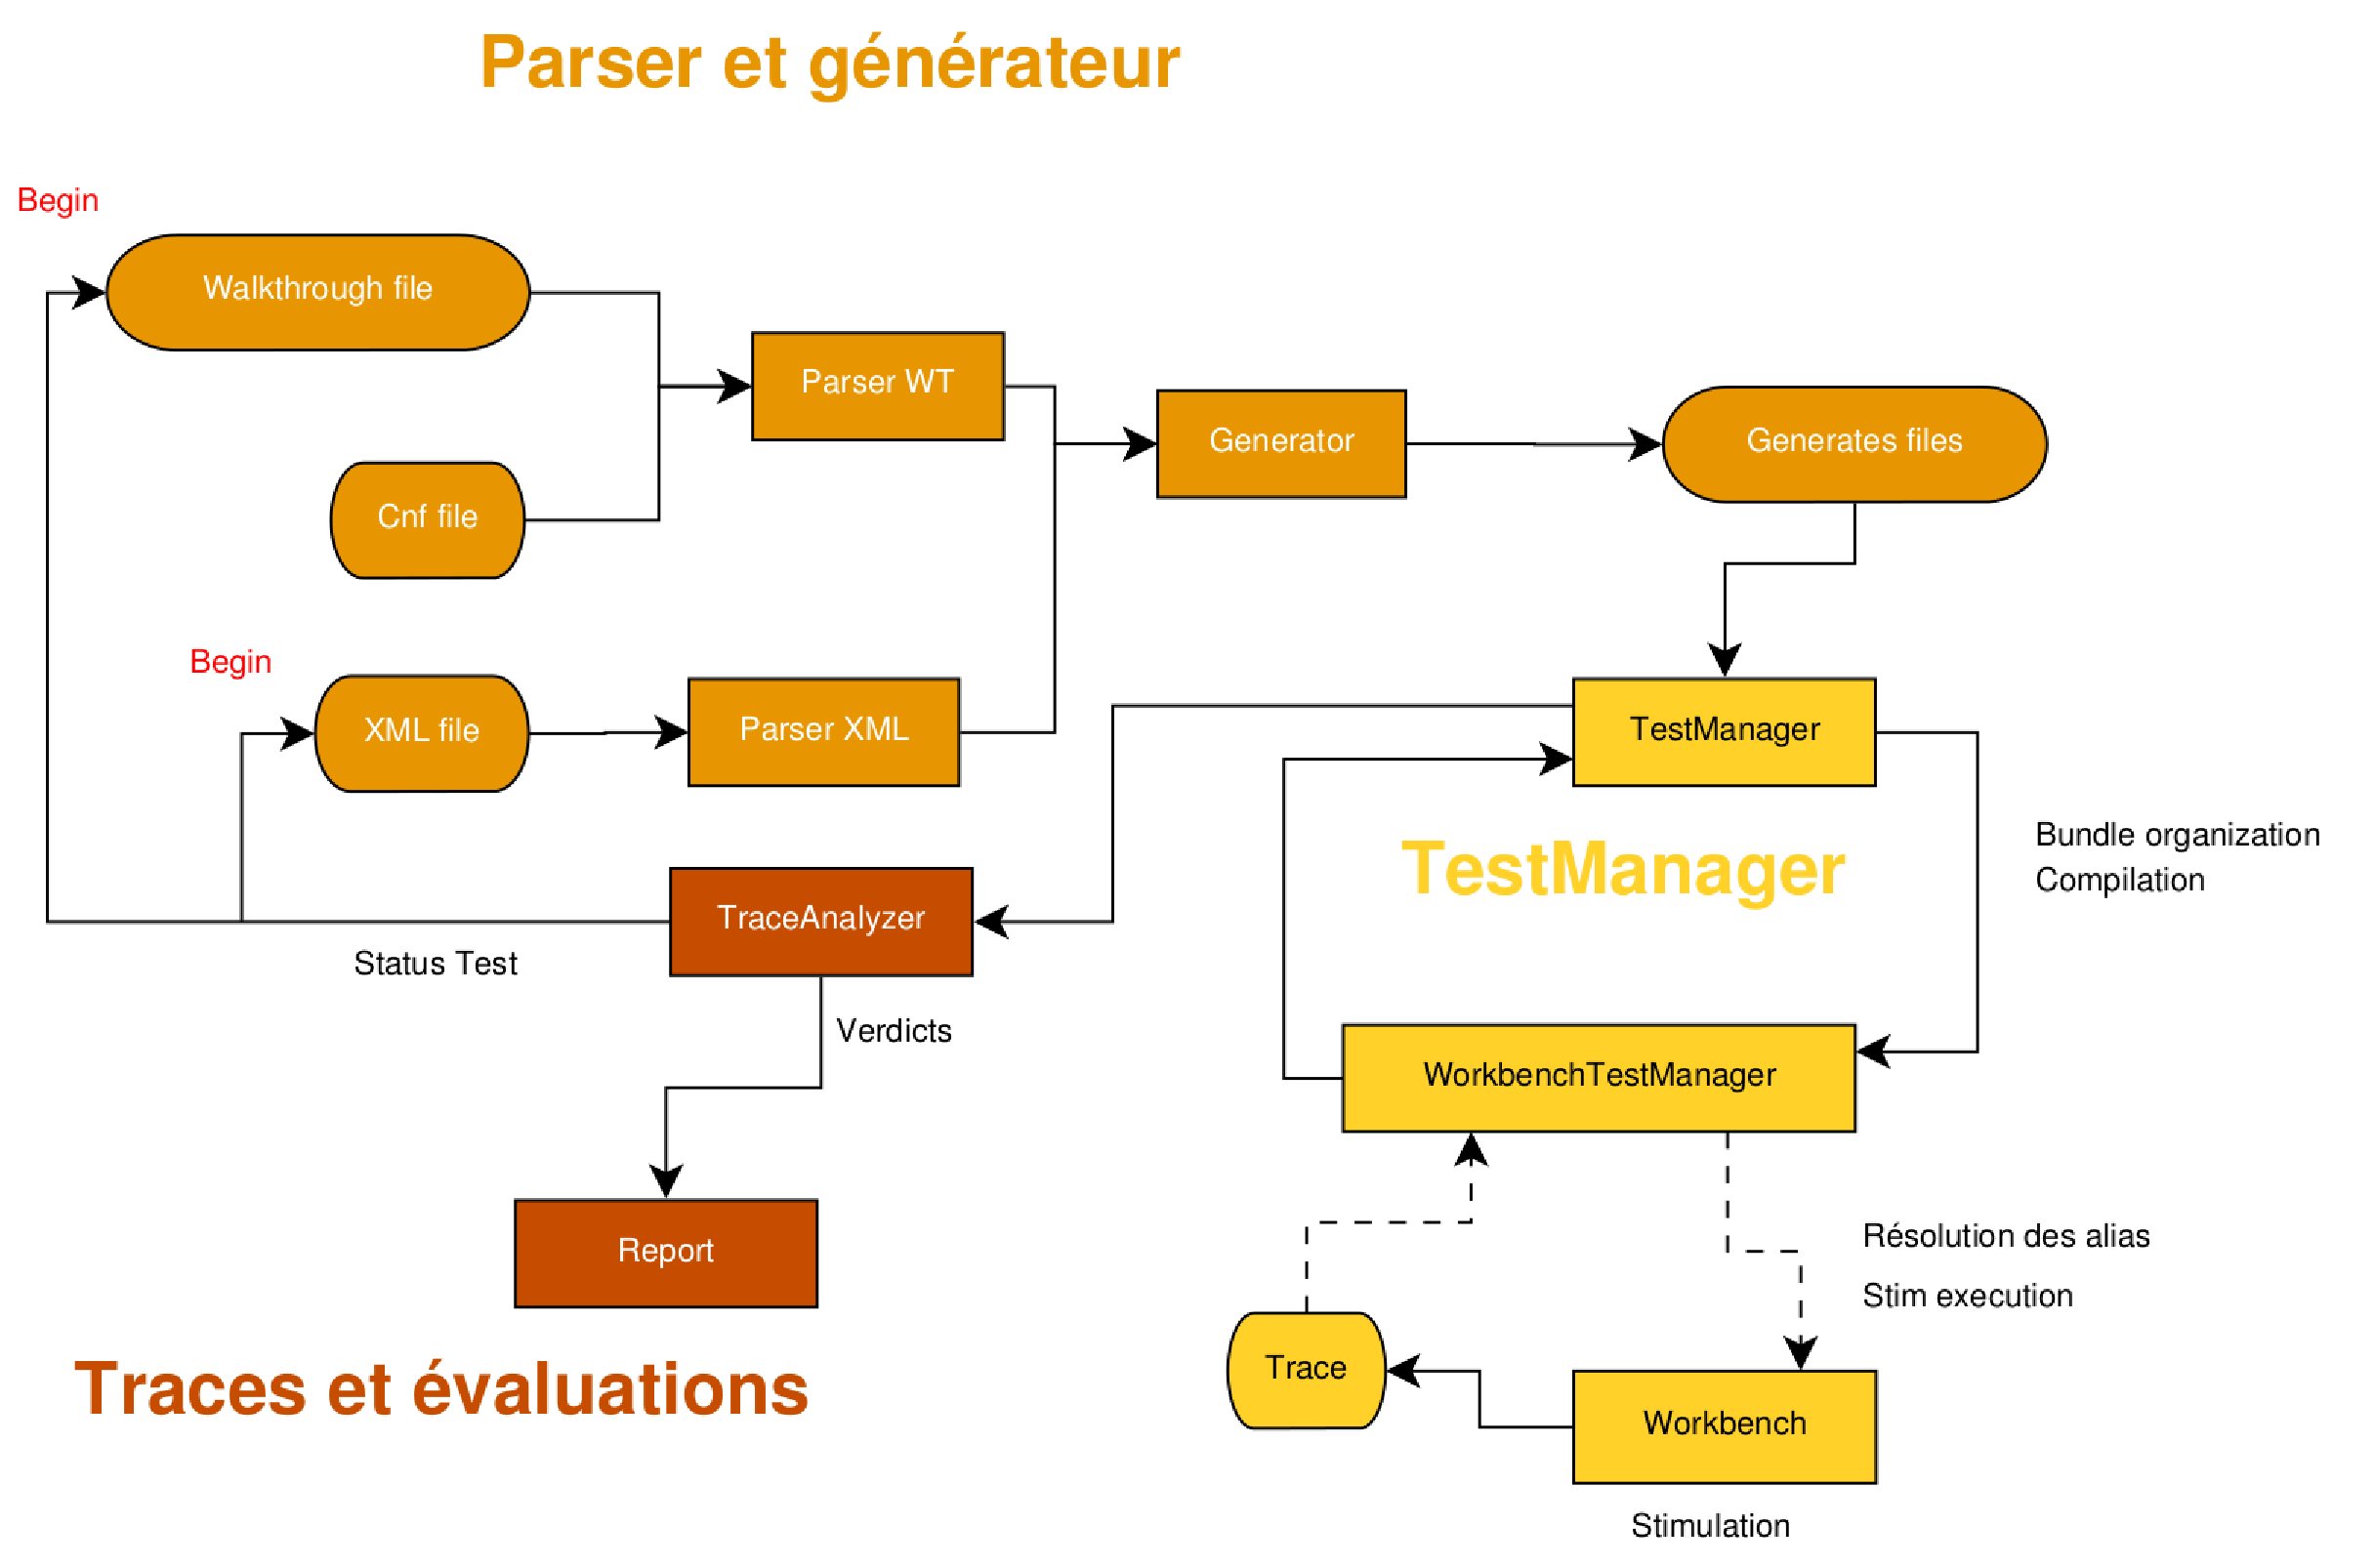
\includegraphics[width=10cm]{generalDiag.eps}
		\caption{Schéma de fonctionnement général}
	\end{figure}
	}
\end{frame}
\begin{frame}[plain]
\begin{tikzpicture}[remember picture,overlay]
\node[at=(current page.center)] {
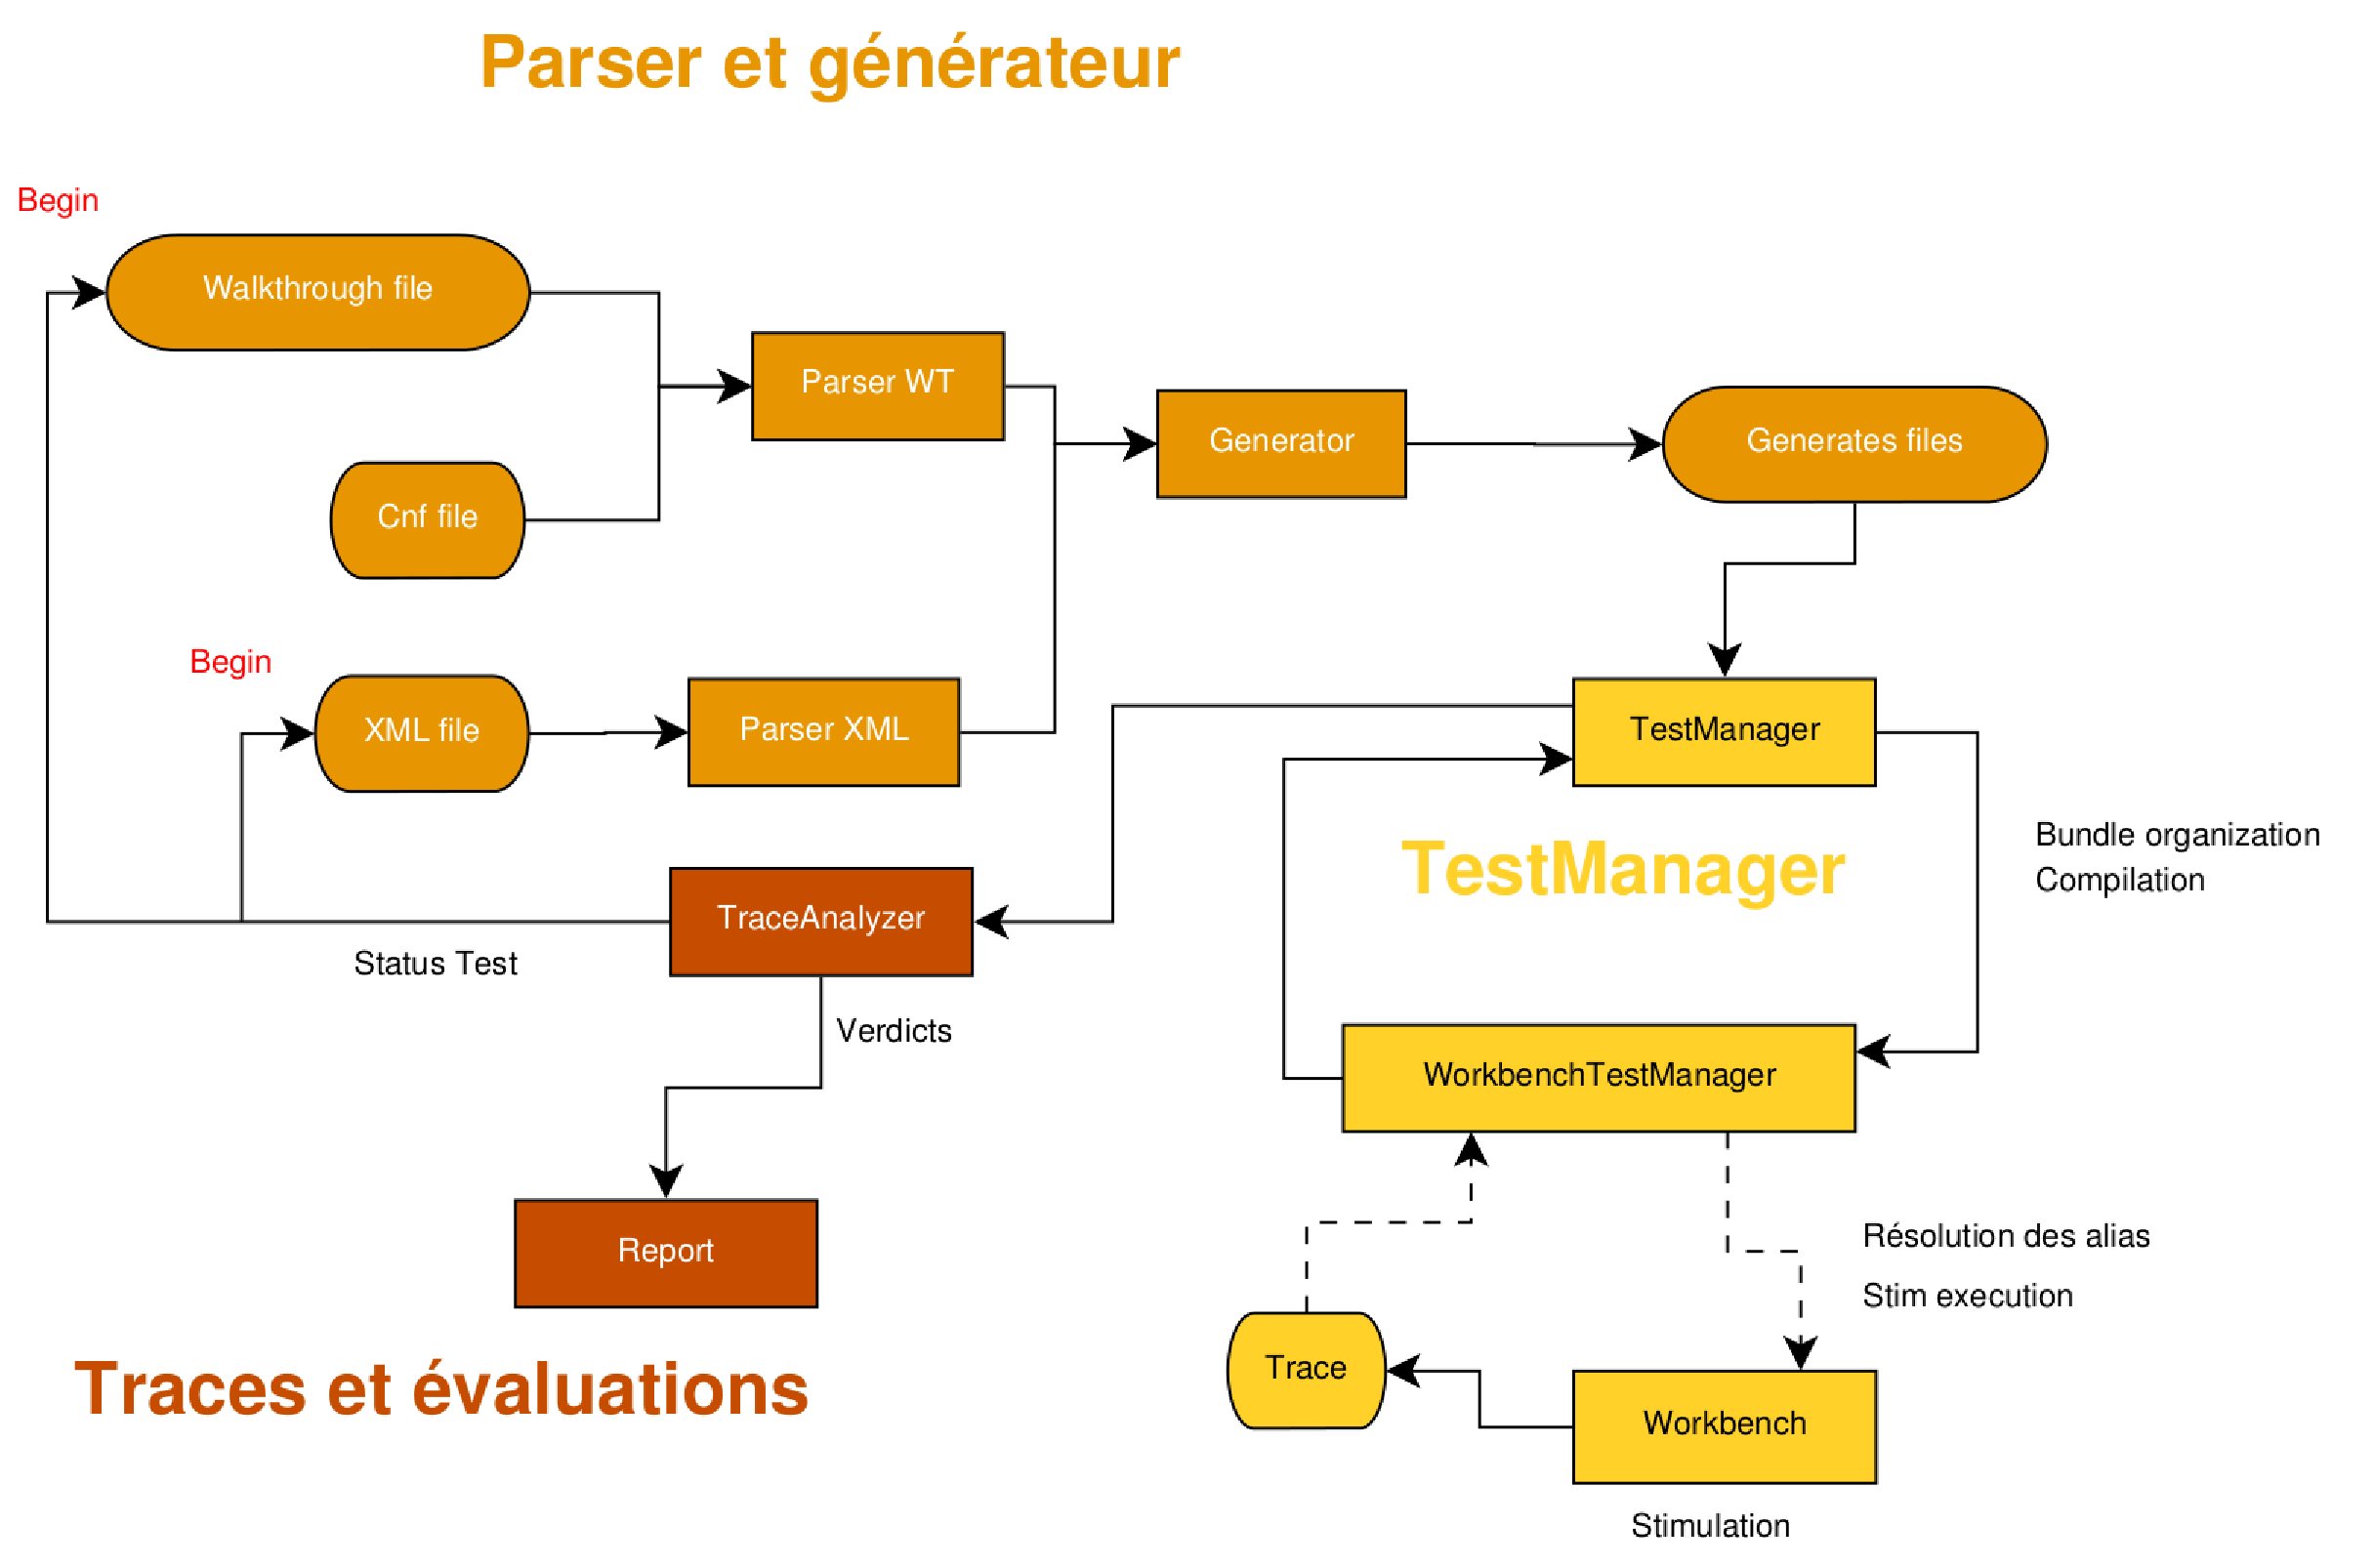
\includegraphics[width=\paperwidth]{generalDiag.eps}
};
\end{tikzpicture}
\end{frame}
\subsection{Parser et g\'en\'erateur}
\begin{frame}{Parser : utilisation de Antlr}
~\vspace{-30px}
\begin{wrapfigure}{r}{1.5cm}
	
\includegraphics[width=1.5cm]{antlr.jpg}
\end{wrapfigure}
	\vspace{-20px}
	\begin{itemize}
		\item Création de 2 grammaires 
			\begin{itemize}
				\item Scénarios et \textit{Excepted Behavior}
				\item Arbre d'évaluation généré automatiquement par Antlr
			\end{itemize}
		\item Parcours de l'arbre. 
			\begin{itemize}
				\item Appel du générateur
				\item Utilise les n\oe{}uds pour connaître le contexte\newline 
				\scriptsize Exemple : \texttt{CHECK(HIL\_VB = 13, TOLRES(1))}
			\end{itemize}
	\end{itemize}
	\begin{figure}[h]
		\centering
		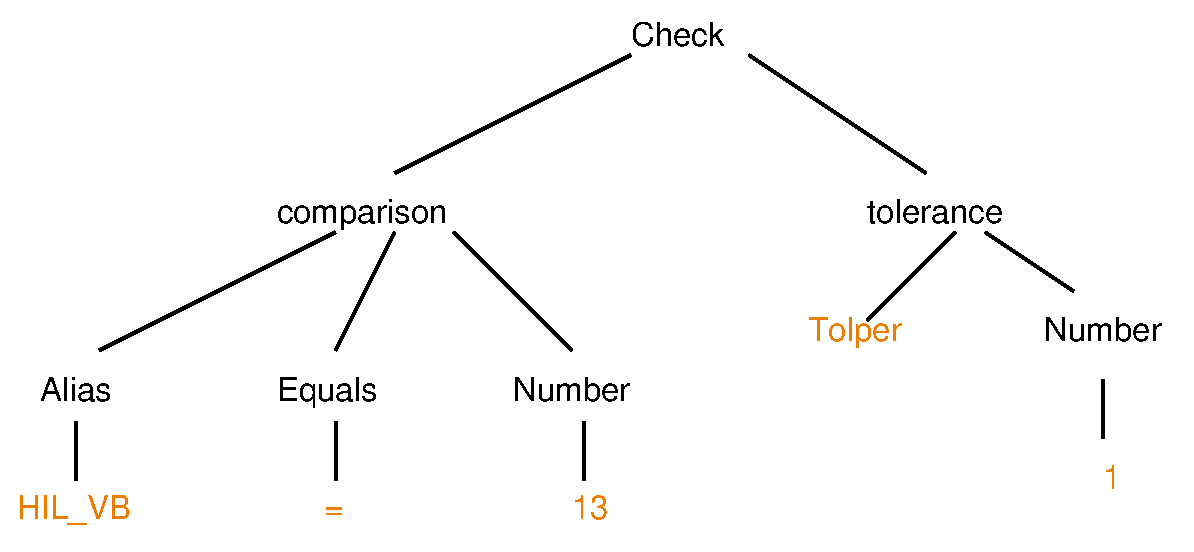
\includegraphics[width=6cm]{treeCheck.eps}
		\caption{Exemple d'arbre d'évaluation}
	\end{figure}
	\end{frame}
	\begin{frame}{Gestion des exceptions}
	\footnotesize
	Avant la phase d'exécution des tests: 
	\normalsize
			\begin{itemize}
					\vspace{-10px}
		\item Erreur de syntaxe
		\item Écriture sur une variable en lecture seule
		\item Lecture sur une variable en écriture seule
		\item Variable inconnue 
		\end{itemize}
\end{frame}

\begin{frame}{Générateur : utilisation de Freemarker}
	~
	\begin{wrapfigure}{r}{1.5cm}
		
\includegraphics[width=1.5cm]{FreeMaker.png}
	\end{wrapfigure}
	\vspace{-30px}
	\begin{itemize}
		\item Système de template : Freemarker
			\vfill
			\pause
		\item 3 types de classes Java à générer
		\begin{itemize}
			\item \texttt{PrecondStim}
			\item \texttt{StimScénario}
			\item \texttt{GreenTTest} $\rightarrow$ Contient \textit{ExpectedBehavior}, informations du rapport, \ldots
		\end{itemize}
		\begin{figure}[H]
			\centering
			\includegraphics[width=8cm]{test.eps}
		\end{figure}
			\vfill
		\pause
		\item Générer du code qui sera compilé\newline
			$\rightarrow$ Limiter les erreurs
	\end{itemize}
\end{frame}

\section*{Conclusion}
\begin{frame}{Vers le master Développement Logiciel}
		Bilan pour Continental:
	\vspace{-10px}
	\begin{itemize}[<+->]
		  \setbeamercovered{transparent}
			\item Stage prolongé jusqu'à mi-juillet
			\item Participation à la conception $\rightarrow$ Regard neuf
			\item Développement de différents modules 
				\begin{itemize}
					\item<3->Parser et génération des scénarios: terminés
					\item<3-> Génération des
						\textit{ExpectedBehavior} : en cours
					\item<3-> Analyse des traces, rapport détaillé : à faire
				\end{itemize}
			\item Plateforme à destination d'une vingtaine de
				projets\newline
				$\rightarrow$ Centaines de milliers de véhicules
		\end{itemize}
\end{frame}
\begin{frame}{Vers le master Développement Logiciel}
		\vfill
	Bilan personnel:
	\vspace{-10px}
		\begin{itemize}[<+->]
		  \setbeamercovered{transparent}
			\item D'un point de vue technique
				\begin{itemize}
					\item Expérience en conception logicielle
						\scriptsize
						\newline $\rightarrow$ UML, design patterns
					\item Différentes visions d'un problème
				\end{itemize}
		\vfill
			\item D'un point de vue humain
				\begin{itemize}
					\item Travail en équipe
					\item Synthèse et restitutions
				\end{itemize}
		\end{itemize}
		\vfill
\end{frame}
\begin{frame}{Avez-vous des questions ?}
	\begin{figure}[H]
		\centering
		
\includegraphics[width=3.5cm]{interrogation.jpg}
	\end{figure}
\end{frame}
\end{document}


%Intro 2'
%Entreprise
	% 1'
	% 2'
%probleme
	% 2'
%greent
	% 2.5'
	% 4'
%conclu 
	% 2'

%15.5

% gestion des ex ->
%	rédac -> crreeer
